\documentclass[oneside,a4paper,11pt]{article} 
\usepackage{fontspec}
\usepackage{natbib}
\usepackage{booktabs}
\usepackage{xltxtra} 
\usepackage{polyglossia} 
\usepackage[table]{xcolor}
\usepackage{tikz}
\usetikzlibrary{trees}
\usepackage{gb4e} 
\usepackage{multicol}
\usepackage{graphicx}
\usepackage{float}
\usepackage{hyperref} 
\hypersetup{bookmarks=false,bookmarksnumbered,bookmarksopenlevel=5,bookmarksdepth=5,xetex,colorlinks=true,linkcolor=blue,citecolor=blue}
\usepackage[all]{hypcap}
\usepackage{memhfixc}
\usepackage{lscape} 
 \usepackage{multicol}
 \usepackage{amssymb}
%\setmainfont[Mapping=tex-text,Numbers=OldStyle,Ligatures=Common]{Charis SIL} 
\newfontfamily\phon[Mapping=tex-text,Ligatures=Common,Scale=MatchLowercase]{Charis SIL} 
\newcommand{\ipa}[1]{{\phon\textit{#1}}} 
\newcommand{\grise}[1]{\cellcolor{lightgray}\textbf{#1}}
\newfontfamily\cn[Mapping=tex-text,Ligatures=Common,Scale=MatchUppercase]{SimSun}%pour le chinois
\newcommand{\zh}[1]{{\cn #1}}
\newcommand{\Y}{\Checkmark} 
\newcommand{\N}{} 
\newcommand{\zhc}[2]{\zh{#1} \ipa{#2}} 
\newcommand{\refb}[1]{(\ref{#1})}
\newcommand{\tld}{\textasciitilde{}}
\newcounter{exonb}
\newcommand{\exercice}[1]{\noindent%
\begin{center}
\begin{minipage}[t]{.8\textwidth}
\vskip 10pt 
\rule{\linewidth}{1pt}  
\vskip 10pt 
\stepcounter{exonb} 
\textbf{\centerline{Exercise \Roman{exonb}}}
\vskip 10pt 
\rule{\linewidth}{1pt}  
\indent
#1
\rule{\linewidth}{1pt}  
\end{minipage} 
\end{center}
 }
\newcommand{\exo}[2]{\noindent%
\begin{center}
\begin{minipage}[t]{.8\textwidth}
\vskip 10pt 
\rule{\linewidth}{1pt}  
\vskip 10pt 
\stepcounter{exonb} 
\textbf{\centerline{Exercise \Roman{exonb}}}
\vskip 10pt 
\rule{\linewidth}{1pt}  
\indent
#1
\vskip 10pt
\begin{multicols}{3}
#2
\end{multicols}
\rule{\linewidth}{1pt}  
\end{minipage} 
\end{center}
 }
\newcommand{\translit}[1]{$\langle$#1$\rangle$}
\newcommand{\zhd}[2]{\begin{tabular}{l}
\zh{#1}\\
\ipa{#2}\\
\end{tabular}}
 \newcommand{\bleu}[1]{{\color{blue}#1}}
\newcommand{\rouge}[1]{{\color{red}#1}} 
\newcommand{\verte}[1]{{\textbf{#1}}}
\XeTeXlinebreaklocale "zh" %使用中文换行 
\XeTeXlinebreakskip = 0pt plus 1pt % 

 \begin{document} 
\title{Middle Chinese}
\author{Guillaume Jacques\\ CNRS-CRLAO-INALCO}
\maketitle

\section{Early Middle Chinese} \label{sec:emc}

\subsection{Transcribing vs reconstructing MC}

\subsubsection{Consonants}
\begin{table}[H]
\caption{Early Middle Chinese initial consonants} \label{tab:mc.onset}
\begin{tabular}{llllllllllllllll}
\toprule
 	\zhc{幫}{p} & 	\zhc{滂}{pʰ} & 	\zhc{並}{b} & 	\zhc{明}{m} & 	 & 	 & (\zh{喻}_3/\zhc{云}{w})	 & 	\\
  	\zhc{端}{t} & 	\zhc{透}{tʰ} & 	\zhc{定}{d} & 	\zhc{泥}{n} & 	 & 	 & 	 & 	\\
 	\zhc{知}{ʈ} & 	\zhc{徹}{ʈʰ} & 	\zhc{澄}{ɖ} & 	\zhc{娘}{ɳ} & 	 & 	 & 	 & 	\\
  	 & 	 & 	 & 	 & 	 & 	 & 	\zhc{來}{l} & 	\\
  	\zhc{精}{ts} & 	\zhc{清}{tsʰ} & 	\zhc{從}{dz} & 	 & 	\zhc{心}{s} & 	\zhc{邪}{z} & 	 & 	\\
  	\zh{照}_2/\zhc{莊}{tʂ} & 	\zh{穿}_2/\zhc{初}{tʂʰ} & 	\zh{牀}_2/\zhc{崇}{dʐ} & 	 & 	  	\zh{審}_2/\zhc{生}{ʂ} & 	 \zh{禪}_2\ipa{ʐ} & 	 & 	\\
 	  	\zh{照}_3/\zhc{章}{tɕ} & 	\zh{穿}_3/\zhc{昌}{tɕʰ} & 	\zh{禪}_3/\zhc{禪}{dʑ} & 	\zhc{日}{ɲ} & 	\zh{審}_3/\zhc{書}{ɕ} & 	\zh{牀}_3/\zhc{船}{ʑ} & 	\zh{喻}_4/\zhc{以}{j} & 	\\
 	\zhc{見}{k} & 	\zhc{溪}{kʰ} & 	\zhc{群}{ɡ(j)} & 	\zhc{疑}{ŋ} & 	 & 	 & 	 & 	\\
 	\zhc{影}{ʔ} & 	 & 	 & 	 & 	\zhc{曉}{x} & 	\zhc{匣}{ɣ} & 	 & 	\\
\bottomrule
\end{tabular}
\end{table}

Final consonants: \ipa{-p},  \ipa{-t},  \ipa{-k},  \ipa{-m},  \ipa{-m},  \ipa{-ŋ}, \ipa{-j}, \ipa{-w}.

Baxter's (\citeyear{baxter92}) typeable transcription: 
\begin{enumerate}
\item Retroflex consonants: \ipa{ʈ} = \translit{tr}, \ipa{tʂʰ}  =  \translit{tsrh} 
\item Alveolo-Palatal consonants: \ipa{tɕ} = \translit{tsy}
\item Velars: \ipa{ŋ} = \translit{ng}, \ipa{ɣ} = \translit{h}
\item Glides: \ipa{j} = \translit{y-}, \ipa{w} = \translit{hjw-} (contrast between \zhc{越}{hjwot}  and \zhc{悦}{jwet}).
\end{enumerate}

Marginal initials:
\begin{itemize}
\item 
(\zh{喻}_3/\zh{云} initial only appears with \zhc{合口}{hékǒu} syllables, except for \zhc{焉}{hjen} and \zhc{矣}{hi}).
\item The \ipa{ʐ} initial only attested in two characters (including \zhc{俟}{ʐiX}).
\end{itemize}

\subsubsection{Rhymes} \label{sec:rhymes}

The four divisions in Baxter's transcription:
\begin{enumerate}
\item \ipa{-a}, \ipa{-o}, \ipa{-u}
\item \ipa{-ɛ}, \ipa{-æ}
\item palatal+V, \ipa{-jV}, \ipa{-i} (V $\in$\{\ipa{a}, \ipa{æ}, \ipa{o}, \ipa{u},  \ipa{i}, \ipa{e}, \ipa{ɨ}\})
\item \ipa{-e}
\end{enumerate}

Medial \ipa{-w} in \zhc{合口}{hékǒu} syllables, except (i) if the main vowel is not \ipa{u} or \ipa{o+w} (ii) the initial consonant is not a labial, unless the \zhc{合口}{hékǒu} rhyme has a different name than its \zhc{開口}{kāikǒu} equivalent, such as \zhc{咍}{-oj} vs \zhc{灰}{-woj} (for instance \zhc{陪}{bwoj}, see Table \ref{tab:xie.zhi}).

\subsubsection{Tones}

\begin{tabular}{lll} 
\zhc{平}{bjæŋ} & \zhc{端}{twan} \\
\zhc{上}{dʑaŋX} & \zhc{短}{twanX} \\
\zhc{去}{kʰjoH} & \zhc{段}{twanH} \\
\zhc{入}{ɲip} & \zhc{掇}{twat} \\
\end{tabular}

\subsubsection{Subclasses of third division} \label{sec:third}

According to \citet{lirong56qy}, third division rhymes are classified into three groups:

\begin{itemize}
\item \zhc{子}{zǐ}: Only found with grave initials (labial, velar or guttural)
\item \zhc{丑}{chǒu}: Compatible with all places of articulation except dental stops, no \zhc{重紐}{chóngniǔ} distinction.
\item \zhc{寅}{yín}: Compatible with all places of articulation except dental stops, division between \zhc{重紐}{chóngniǔ} 3 and 4 (this terminology is explained in section \ref{sec:yuntu}). \zhc{重紐}{chóngniǔ} 4 rhymes are transcribed by Baxter with an additional \ipa{-i-} (if the main vowel is not \ipa{i}) or an additional \ipa{-j-}(if the main vowel is \ipa{i}).
\end{itemize} 

\begin{table}[H]
\caption{\zhc{果}{guǒ}, \zhc{假}{jiǎ} and \zhc{遇}{yù}} \centering \label{tab:guo}
\begin{tabular}{llllll}
\toprule
Rhyme & Division & & Transcription \\
\midrule
\zh{歌} &	I &	&	\ipa{-a} &	\\
\zh{戈} &	I &	&	\ipa{-wa} &	\\
\zh{戈} &	III &	\zh{丑} &	\ipa{-j(w)a} &	\\
\midrule
\zh{麻} &	II &	&	\ipa{-(w)æ} &	\\
\zh{麻} &	III &	\zh{丑} &	\ipa{-jæ} &	\\
\midrule
\zh{模} &	I &	&	\ipa{-u} &	\\
\zh{魚} &	III &	\zh{丑} &	\ipa{-jo} &	\\
\zh{虞} &	III &	\zh{丑} &	\ipa{-ju} &	\\
\bottomrule
\end{tabular}
\end{table}


\begin{table}[H]
\caption{\zhc{蟹}{xiè} and \zhc{止}{zhǐ} (\ipa{-j} coda)} \centering \label{tab:xie.zhi}
\begin{tabular}{llllll}
\toprule
Rhyme & Division & & Transcription \\
\midrule
\zh{咍} &	I &	&	\ipa{-oj} &	\\
\zh{灰} &	I &	&	\ipa{-woj} &	\\
\zh{泰} &	I &	&	\ipa{-(w)ajH} &	\\
\zh{皆} &	II &	&	\ipa{-(w)ɛj} &	\\
\zh{佳} &	II &	&	\ipa{-(w)ɛɨ} &	\\
\zh{夬} &	II &	&	\ipa{-(w)æjH} &	\\
\zh{祭} &	III &	\zh{寅} &	\ipa{-j(w)(i)ejH} &	\\
\zh{廢} &	III &	\zh{子} &	\ipa{-j(w)ojH} &	\\
\zh{齊} &	IV &	&	\ipa{-(w)ej} &	\\
\midrule
\zh{支} &	III &	\zh{寅} &	\ipa{-j(w)(i)e} &	\\
\zh{脂} &	III &	\zh{寅} &	\ipa{-(j)(w)ij} &	\\
\zh{之} &	III &	\zh{丑} &	\ipa{-i} &	\\
\zh{微} &	III &	\zh{子} &	\ipa{-j(w)ɨj} &	\\
\bottomrule
\end{tabular}
\end{table}


\begin{table}[H]
\caption{\zhc{效}{xiào} and \zhc{流}{liú} (\ipa{-w} coda)} \centering \label{tab:xiao}
\begin{tabular}{llllll}
\toprule
Rhyme & Division & & Transcription \\
\midrule
\zh{豪} &	I &	&	\ipa{-aw} &	\\
\zh{肴} &	II &	&	\ipa{-æw} &	\\
\zh{宵} &	III &	\zh{寅} &	\ipa{-j(i)ew} &	\\
\zh{蕭} &	IV &	&	\ipa{-ew} &	\\
\zh{侯} &	I &	&	\ipa{-uw} &	\\
\zh{尤} &	III &	\zh{丑} &	\ipa{-juw} &	\\
\zh{幽} &	III &	\zh{丑}=\zh{重紐}4 &	\ipa{-jiw} &	\\
\bottomrule
\end{tabular}
\end{table}


\begin{table}[H]
\caption{\zhc{咸}{xián} and \zhc{深}{shēn} (\ipa{-m} coda)} \centering \label{tab:xian}
\begin{tabular}{llllll}
\toprule
Rhyme & Division & & Transcription \\
\midrule
\zh{覃} &	I &	 &	\ipa{-om} &	\\
\zh{談} &	I &	 &	\ipa{-am} &	\\
\zh{咸} &	II &	 &	\ipa{-ɛm} &	\\
\zh{銜} &	II &	 &	\ipa{-æm} &	\\
\zh{鹽} &	III &	\zh{寅} &	\ipa{-j(i)em} &	\\
\zh{嚴} &	III &	\zh{子} &	\ipa{-jæm} &	\\
\zh{凡} &	III &	\zh{子} &	\ipa{-jom} &	\\
\zh{添} &	IV &	 &	\ipa{-em} &	\\
\midrule
\zh{侵} &	III &	\zh{寅} &	\ipa{-(j)im} &	\\
\bottomrule
\end{tabular}
\end{table}

\begin{table}[H]
\caption{\zhc{山}{shān} and \zhc{臻}{zhēn} (\ipa{-n} coda)} \centering \label{tab:shan}
\begin{tabular}{llllll}
\toprule
Rhyme & Division & & Transcription \\
\midrule
\zh{寒} & 	I & 	& 	\ipa{-an} & 	\\
\zh{桓} & 	I & 	& 	\ipa{-wan} & 	\\
\zh{刪} & 	II & 	& 	\ipa{-(w)æn} & 	\\
\zh{山} & 	II & 	& 	\ipa{-(w)ɛn} & 	\\
\zh{仙} & 	III & 	\zh{寅} & 	\ipa{-j(i)(w)en} & 	\\
\zh{元} & 	III & 	\zh{子} & 	\ipa{-j(w)on} & 	\\
\zh{先} & 	IV & 	& 	\ipa{-(w)en} & 	\\
\midrule
\zh{痕} & 	I & 	& 	\ipa{-on} & 	\\
\zh{魂} & 	I & 	& 	\ipa{-won} & 	\\
\zh{臻} & 	III & 	\zh{丑} & 	\ipa{-in} & 	\\
\zh{眞} & 	III & 	\zh{寅} & 	\ipa{-(j)(w)in} & 	\\
\zh{欣} & 	III & 	\zh{子} & 	\ipa{-jɨn} & 	\\
\zh{文} & 	III & 	\zh{子} & 	\ipa{-jun} & 	\\
\bottomrule
\end{tabular}
\end{table}


\begin{table}[H]
\caption{\zhc{宕}{dàng}, \zhc{江}{jiāng}, \zhc{曾}{zēng}, \zhc{梗}{gěng} and \zhc{通}{tōng} (\ipa{-ŋ} coda)} \centering \label{tab:dang}
\begin{tabular}{llllll}
\toprule
Rhyme & Division & & Transcription \\
\midrule
\zh{唐} & 	I & 	& 	\ipa{-(w)aŋ} & 	\\
\zh{陽} & 	III & 	\zh{丑} & 	\ipa{-j(w)aŋ} & 	\\
\midrule
\zh{江} & 	II & 	& 	\ipa{-æwŋ} & 	\\
\midrule
\zh{登} & 	I & 	& 	\ipa{-(w)oŋ} & 	\\
\zh{蒸} & 	III & 	\zh{丑} & 	\ipa{-iŋ} & 	\\
\midrule
\zh{庚} & 	II & 	& 	\ipa{-(w)æŋ} & 	\\
\zh{耕} & 	II & 	& 	\ipa{-(w)ɛŋ} & 	\\
\zh{庚} & 	III & 	\zh{子}=\zh{重紐3} & 	\ipa{-j(w)æŋ} & 	\\
\zh{清} & 	III & 	\zh{寅} & 	\ipa{-j(w)(i)eŋ} & 	\\
\zh{青} & 	IV & 	& 	\ipa{-(w)eŋ} & 	\\
\midrule
\zh{東} & 	I & 	& 	\ipa{-uwŋ} & 	\\
\zh{冬} & 	I & 	& 	\ipa{-owŋ} & 	\\
\zh{東} & 	III & 	\zh{丑} & 	\ipa{-juwŋ} & 	\\
\zh{鍾} & 	III & 	\zh{丑} & 	\ipa{-jowŋ} & 	\\
\bottomrule
\end{tabular}
\end{table}


 \exo{Indicate the initial consonant, the division, the rhyme and the tone of the following characters}{
\zhc{睹}{tuX}

\zhc{塵}{ɖin} %ɖ, 3, -in, ping

\zhc{炒}{tʂʰæwX} %tʂʰ, 2, -æw, shang

\zhc{朝}{ɖjew} %ɖ, 3, -jew, ping

\zhc{吹}{tɕʰwe} %tɕʰ, 3, -w-, -je, ping

\zhc{畜}{ʈʰjuwk} 

\zhc{鄧}{doŋH} 

\zhc{妃}{pʰjɨj} 

\zhc{範}{bjomX} 

\zhc{彪}{pjiw} 

\zhc{餅}{pjieŋX} 

\zhc{兒}{ɲe} 

\zhc{競}{gjæŋH}

\zhc{脈}{mɛk} 
 
\zhc{汪}{ʔwaŋ} 
 
\zhc{驗}{ŋjemH} 
  
\zhc{王}{hjwaŋ} 
  
\zhc{緣}{jwen}
}

 \exo{Using the electronic Guangyun, indicate the MC reading(s)  of the following characters}{\cn
 揭 
 上
 民
 永
 嫩
 龍
 日
 復
 不
 藏
 斷
 }
\subsection{Complementary distributions}

 \begin{table}[H]
 \caption{Complementary distribution between initial consonants and divisions, rhymes with \ipa{-ŋ} coda} \centering
\begin{tabular}{l|llllll}
\toprule
&\zhc{搨}{-aŋ}& \zhc{庚}{-æŋ} & \zhc{陽}{-jaŋ} &\zhc{青}{-eŋ} \\
\midrule
\zhc{端}{t} 	&	\zhc{當}{taŋ} 	& \grise{}	& \grise{}	&	\zhc{丁}{teŋ}  \\
\zhc{知}{ʈ} 	&	\grise{}&\zhc{趟}{ʈæŋ} 	&	\zhc{張}{ʈjaŋ} 	&	\grise{}	&		\\
\zhc{精}{ts} 	&	\zhc{臧}{tsaŋ} &\grise{}	&	\zhc{將}{tsjaŋ} 	&	\zhc{菁}{tseŋ} 	&		\\
\zhc{莊}{tʂ} 	&	\grise{}&\zhc{鎗}{tʂʰæŋ} 	& \zhc{莊}{tʂjaŋ} 	&		\grise{}&		\\
\zhc{章}{tɕ} 	&		\grise{}&		\grise{}&	\zhc{章}{tɕaŋ} 	&		\grise{} 		\\
\zhc{幫}{p} 	&	\zhc{幫}{paŋ} 	&	\zhc{彭}{bæŋ} 	&	\zhc{方}{pjaŋ} 	&	\zhc{瓶}{beŋ}\\
\zhc{見}{k} 	&	\zhc{剛}{kaŋ} 	&	\zhc{庚}{kæŋ} 	&	\zhc{薑}{kjaŋ} 	&	\zhc{經}{keŋ} 	\\
\bottomrule
\end{tabular}
\end{table}


 \begin{table}[H]
 \caption{Complementary distribution between initial consonants and divisions, rhymes with \ipa{-w} coda} \centering
\begin{tabular}{l|llllll}
\toprule
&\zhc{豪}{-aw}& \zhc{爻}{-æw} & \zhc{宵}{-jew} &\zhc{萧}{-ew} \\
\midrule
\zhc{端}{t} 	&	\zhc{刀}{taw} 	& \grise{}	& \grise{}	&	\zhc{雕}{tew}  \\
\zhc{知}{ʈ} 	&	\grise{}&\zhc{啁}{ʈæw} 	&	\zhc{朝}{ʈjew} 	&	\grise{}	&		\\
\zhc{精}{ts} 	&	\zhc{遭}{tsaw} &\grise{}	&	\zhc{焦}{tsjew} 	&	\zhc{湫}{tsewX} 	&		\\
\zhc{莊}{tʂ} 	&	\grise{}&\zhc{抓}{tʂæw} 	& X	&		\grise{}&		\\
\zhc{章}{tɕ} 	&		\grise{}&		\grise{}&	\zhc{昭}{tɕew} 	&		\grise{} 		\\
\zhc{幫}{p} 	&	\zhc{褒}{paw} 	&	\zhc{包}{pæw} 	&	\zhc{膘}{pjew} 	&	X	\\
\zhc{見}{k} 	&	\zhc{高}{kaw} 	&	\zhc{交}{kæw} 	&	\zhc{驕}{kjew} 	&	\zhc{澆}{kew} 	\\
%\zhc{來}{l} 	&	\zhc{牢}{law} 	&	\grise{}	&	\zhc{療}{ljewH} 	&	\zhc{寥}{lew} 	\\
\bottomrule
\end{tabular}
\end{table}

The orthographic rules of the Baxter transcription integrate some of these complementary distributions; for instance, since fourth division rhymes (\ipa{-eC}) do not appear after palatals, third division rhymes in \ipa{-jeC} are written without the \ipa{-j-} when occurring after those rhymes without risk of confusion (thus \ipa{tɕen} indicates initial \zhc{章}{tɕ-}, rhyme \zhc{仙}{-jen}).

Other particularities:

\begin{itemize}
\item \zhc{來}{l}: nearly no examples in division II.
\item \zhc{子}{zǐ}-class rhymes only compatible with velars, labials and pharyngeals (cf section \ref{sec:third}).
\item \zhc{群}{g-} only in third division.
\end{itemize}


\textbf{Some important exceptions}: \zhc{地}{dijH}, \zhc{打}{tæŋX}, \zhc{冷}{læŋX}


 \exo{Indicate which of the following syllables are impossible in Middle Chinese and why}{ 
\ipa{gen} 
 
\ipa{tʰɛw}

\ipa{tɕæŋ}

\ipa{tʰjij}

\ipa{ɖaŋ}

\ipa{ju}

\ipa{tɕaw}

\ipa{tʂi}

\ipa{ʂu}

\ipa{dʐew}

\ipa{dʐaŋ}

\ipa{bjew}

\ipa{zæw}

\ipa{tɕʰu}

\ipa{ʈu}

\ipa{ʈju}

\ipa{ten}

\ipa{gæ}

\ipa{ʈjon}

\ipa{tɕæŋ}

\ipa{piw}
}
\section{From MC to modern Sinitic languages}

\subsection{Late Middle Chinese}

\begin{table}[H]
\caption{The 36 initials} \centering
\begin{tabular}{llllllll}
\toprule
\zhc{幫}{p} & 	\zhc{滂}{pʰ} & 	\zhc{並}{bɦ} & 	\zhc{明}{m} & 	 & 	 & 	 & 	\\
\zhc{非}{f} & 	\zhc{敷}{fʰ} & 	\zhc{奉}{vɦ} & 	\zhc{微}{ɱ} & 	 & 	 & 	 & 	\\
\zhc{端}{t} & 	\zhc{透}{tʰ} & 	\zhc{定}{dɦ} & 	\zhc{泥}{n} & 	 & 	 & 	 & 	\\
\zhc{知}{ʈ} & 	\zhc{徹}{ʈʰ} & 	\zhc{澄}{ɖɦ} & 	\zhc{娘}{ɳ} & 	 & 	 & 	 & 	\\
 & 	 & 	 & 	 & 	 & 	 & 	\zhc{來}{l} & 	\\
\zhc{精}{ts} & 	\zhc{清}{tsʰ} & 	\zhc{從}{dzɦ} & 	 & 	\zhc{心}{s} & 	\zhc{邪}{zɦ} & 	 & 	\\
\zhc{照}{tʂ} & 	\zhc{穿}{tʂʰ} & 	\zhc{牀}{dʐɦ} & 	\zhc{日}{ɳʐ} & 	\zhc{審}{ʂ} & 	\zhc{禪}{ʐɦ} & 	 & 	\\
\zhc{見}{k} & 	\zhc{溪}{kʰ} & 	\zhc{群}{gɦ} & 	\zhc{疑}{ŋ} & 	 & 	 & 	 & 	\\
\zhc{影}{ʔ} & 	 & 	 & 	 & 	\zhc{曉}{x} & 	\zhc{匣}{ɣɦ} & 	\zhc{喻}{j} & 	\\
\bottomrule
\end{tabular}
\end{table}

Main consonantal changes between EMC and LMC (evidence is presented in section \ref{sec:amoghavajra}).
\begin{itemize}
\item Breathy voicing
\item Labiodentalization (resulting in a contrast between \ipa{*f} and \ipa{*fʰ}, without a corresponding one between \ipa{*s} and \ipa{*sʰ}, a system unattested elsewhere in the languages of the world with aspirated fricatives, see \citealt{jacques11lingua}).
\item Merger of alveolo-palatals and retroflex affricates and fricatives
\item Fricativization of \ipa{ɲ}
\end{itemize}



\subsection{Nanchang dialect}
\zhc{南昌}{Nánchāng}, a \zhc{贛}{Gàn} dialect (\citealt{sagart93gan}).

\begin{table}[H]
\caption{Correspondences between Middle Chinese and Nanchang} \centering \label{tab:nanchang1}
\begin{tabular}{ll|llll}
\toprule
MC& Nanchang &MC& Nanchang &\\
\midrule
\zhc{東}{tuwŋ}		&	\ipa{tuŋ}^{42}	&	\zhc{鹿}{luwk}		&	\ipa{luk}^{5}	\\
\zhc{懂}{tuwŋX}		&	\ipa{tuŋ}^{213}	&	\zhc{端}{twan}		&	\ipa{tɔn}^{42}	\\
\zhc{棟}{tuwŋH}		&	\ipa{tuŋ}^{55}	&	\zhc{短}{twanX}		&	\ipa{tɔn}^{213}	\\
\zhc{通}{tʰuwŋ}		&	\ipa{tʰuŋ}^{42}	&	\zhc{掇}{twat}		&	\ipa{tɔt}^{5}	\\
\zhc{桶}{tʰuwŋX}		&	\ipa{tʰuŋ}^{213}	&	\zhc{脫}{thwat}		&	\ipa{tʰɔt}^{5}	\\
\zhc{痛}{tʰuwŋH}		&	\ipa{tʰuŋ}^{213}	&	\zhc{團}{dwan}		&	\ipa{tʰɔn}^{24}	\\
\zhc{銅}{duwŋ}		&	\ipa{tʰuŋ}^{24}	&	\zhc{斷}{dwanX}		&	\ipa{tʰɔn}^{31}	\\
\zhc{洞}{duwŋH}		&	\ipa{tʰuŋ}^{31}	&	\zhc{暖}{nwanX}		&	\ipa{lɔn}^{213}	\\
\zhc{讀}{duwk}		&	\ipa{tʰuk}^{5}	&	\zhc{亂}{lwanH}		&	\ipa{lɔn}^{31}	\\
\zhc{聾}{luwŋ}		&	\ipa{luŋ}^{55}	&	\zhc{弄}{luwŋH}		&	\ipa{luŋ}^{31}	\\
\bottomrule
\end{tabular}
\end{table}
 
 \exo{Using the data in Table \ref{tab:nanchang1}, fill the following table and describe the correspondences between MC and Nanchang. Compare with standard Mandarin.}{
 
 

 \begin{tabular}{|l|l|l|l|l|}
 \hline
& \zh{平} & \zh{上} & \zh{去} & \zh{入} \\
 \hline
\zh{端} & &&&\\
 \hline
\zh{透} & &&&\\
 \hline
\zh{定} & &&&\\
 \hline
\zh{泥/來} & &&&\\ 
 \hline
 \end{tabular}
}

 \exo{Using the previous exercise, predict the Nanchang reading of the following characters from their MC (\ipa{-aŋ} $\rightarrow$ \ipa{-ɔŋ} and \ipa{-em} $\rightarrow$ \ipa{-iɛn}):}{
 
 \zhc{躺}{tʰaŋX}
 
 \zhc{燙}{tʰaŋH}
 
 \zhc{糖}{daŋ}

 \zhc{郎}{laŋ}

 \zhc{添}{tʰem}

 \zhc{舔}{tʰemX}

 \zhc{貼}{tʰep}

 \zhc{甜}{dem}

 \zhc{簟}{demX}

 \zhc{疊}{dep} 
 }

\section{Rhyme table philology} 

\subsection{\zhc{反切}{fǎnqiè}} \label{sec:fanqie}

\zhc{陳澧}{Chén lǐ}'s \zhc{繫聯法}{xìliánfǎ}

\subsubsection{\zhc{同用}{tóngyòng}}
\begin{itemize}
\item \zhc{布}{puH} = \zhc{博}{pak}+\zhc{故}{kuH}
\item \zhc{北}{pok} = \zhc{博}{pak}+\zhc{墨}{mok}
\item \zhc{補}{puX} = \zhc{博}{pak}+\zhc{古}{kuX}
\end{itemize}
$\Rightarrow$ \zhc{布}{puH} $\equiv$ \zhc{北}{pok} $\equiv$ \zhc{補}{puX} $\equiv$  \zhc{博}{pak}
\subsubsection{\zhc{互用}{hùyòng} (Symmetry)}
\begin{itemize}
\item \zhc{補}{puX} = \zhc{博}{pak}+\zhc{古}{kuX}
\item \zhc{博}{pak} =  \zhc{補}{puX}+\zhc{各}{kak}
\end{itemize}
$\Rightarrow$  \zhc{補}{puX} $\equiv$  \zhc{博}{pak}
\subsubsection{\zhc{遞用}{dìyòng} (Transitivity)}
\begin{itemize}
\item \zhc{邊}{pen} = \zhc{博}{pak}+\zhc{古}{kuX}
\item \zhc{博}{pak} =  \zhc{補}{puX}+\zhc{各}{kak}
\end{itemize}
$\Rightarrow$  \zhc{邊}{pen} $\equiv$ \zhc{補}{puX} $\equiv$  \zhc{博}{pak}

NB: A \zhc{反切上字}{fǎnqiè shàngzì} character is never used as its own \zhc{反切上字}{fǎnqiè shàngzì}.
 \exo{Establish the \zhc{聲類}{shēnglèi} from the following \zhc{反切}{fǎnqiè} (NB: MC readings are not needed)}{
{\cn  
\noindent
來洛哀切

盧洛乎切

洛盧各切

魯郎古切

郎魯當切

浪來宕切

磊落猥切

落盧各切

掠離灼切

林力尋切

離呂支切

呂力舉切

良呂張切

力林直切

槤里典切

林力尋切

里良止切
}}

 \exercice{Using the Guangyun, explain the distribution of the rhymes \zh{臻} and \zh{眞}. }
 
\subsubsection{\zhc{重紐}{chóngniǔ} }

\begin{itemize}
\item \ipa{min} \zh{武巾}: \zh{珉(玟瑉碈)岷罠閩緡䪸笢旻旼𤸅闅汶㨉忞盿䁕鍲𪃯鈱}
\item \ipa{mjin} \zh{彌鄰}: \zh{民闅䁕泯怋}
\item \ipa{bin} \zh{符巾}:	\zh{貧}
\item \ipa{bjin} \zh{符眞}:	\zh{頻蘋薲嬪㰋玭蠙獱顰𧭹嚬𩴱𦇖𡤉}
\item \ipa{kin} \zh{居銀}: \zh{巾}
\item \ipa{ŋin} \zh{語巾}: \zh{銀㹞狺䖜檭鄞圁誾訔嚚䓄珢䴦垠𪛊泿}
\end{itemize} 


\subsection{\zhc{韻鏡}{Yùnjìng}} \label{sec:yuntu}

{\cn
歸釋音字,一如檢禮部韻,且如得「芳弓」反,先就十陽韻求「芳」字,知屬脣音次清第三位(\ref{fig:ang}),卻歸一東韻(\ref{fig:uwng})尋下「弓」字,便就脣音次清第三位取之,乃知為「豐」字,蓋「芳」字是同音之定位;「弓」字是同韻之對映,歸字之訣大概如是。又如「息中反」嵩,「息」字係仄側聲在職字韻,齒音第二清第四位(\ref{fig:ing}),亦隨「中」字歸一東韻,齒音第二清第四位取之。餘並準之。
\begin{figure}[H]
\centering
\label{fig:ang}
\caption{\zhc{陽}{-jaŋ}}
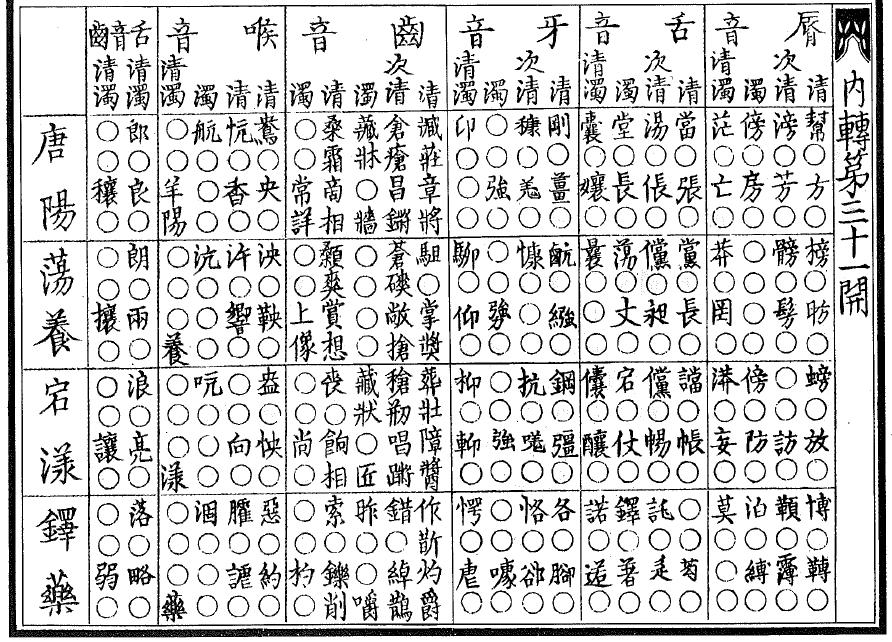
\includegraphics[width=.9\textwidth]{yunjing-ang.jpg}
\end{figure}
\begin{figure}[H]
\centering
\label{fig:uwng}
\caption{\zhc{東}{-uwŋ}}
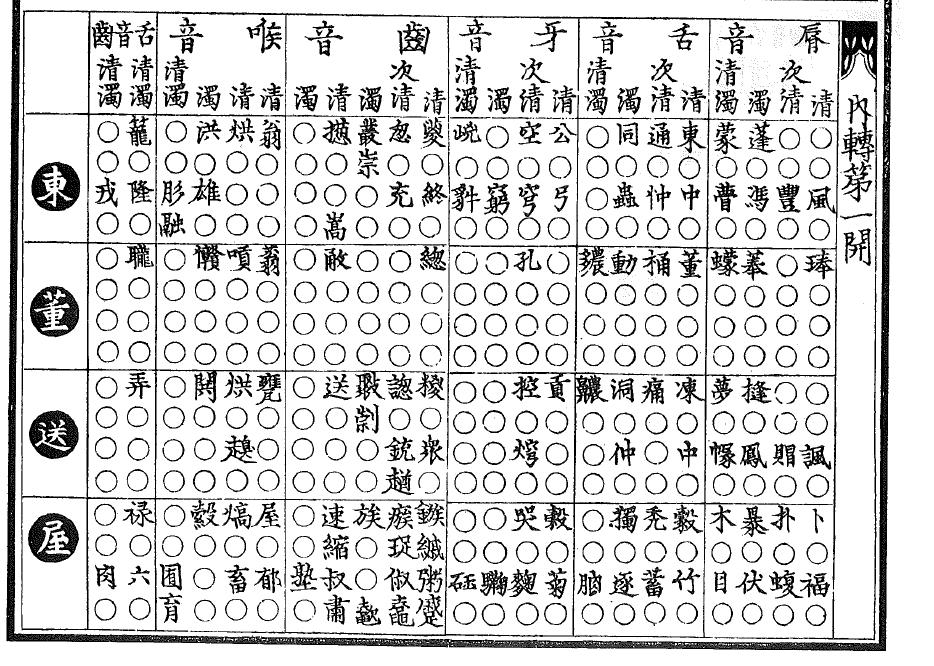
\includegraphics[width=.9\textwidth]{yunjing-uwng.jpg}
\end{figure}

\begin{figure}[H]
\centering
\label{fig:ing}
\caption{\zhc{蒸}{-iŋ}}
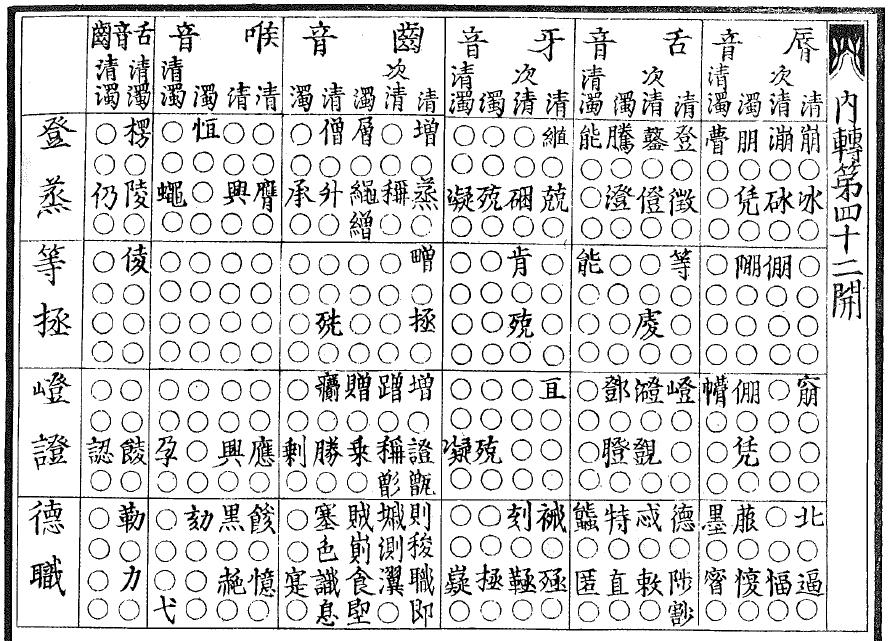
\includegraphics[width=\textwidth]{yunjing-ing.jpg}
\end{figure}

「祖紅反」(\ref{fig:u})歸成「騣」字,雖韻鏡中有洪無紅(\ref{fig:uwng}),檢反切之例,上下二字或取同音,不必正體。

(葼=騣,子紅切)
\begin{figure}[H]
\centering
\label{fig:u}
\caption{\zhc{模}{-u}}
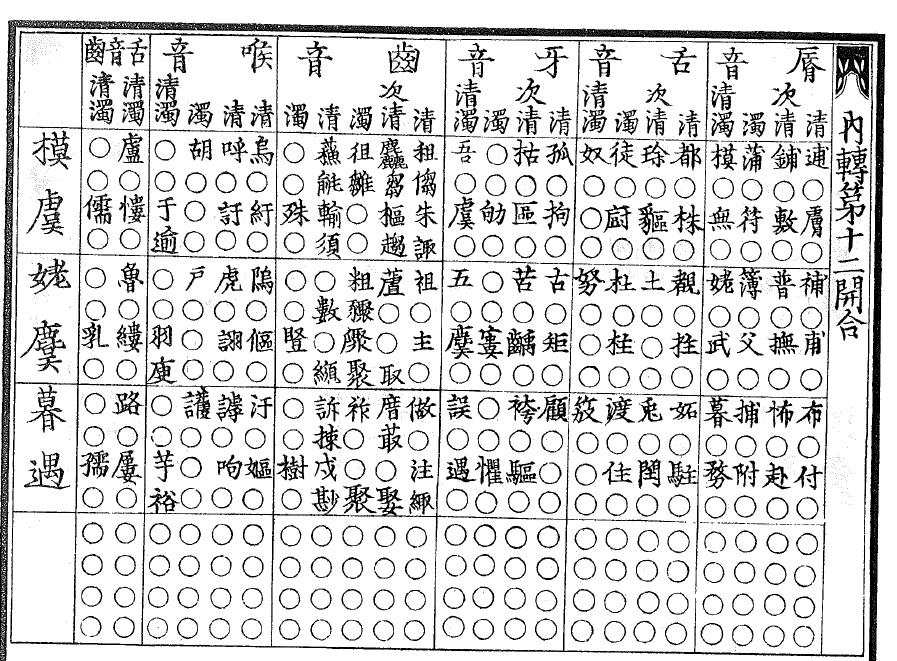
\includegraphics[width=.9\textwidth]{yunjing-u.jpg}
\end{figure}

「慈陵」反「繒」,慈字屬齒音第一濁第四位(\ref{fig:i}),就「蒸」韻歸成「繒」字(\ref{fig:ing}),而「陵」字又不相映,蓋逐韻屬單行字母者,上下聯續二位只同一音,此第四圍亦「陵」字音也。餘準此。

\begin{figure}[H]
\centering
\label{fig:i}
\caption{\zhc{之}{-i}}
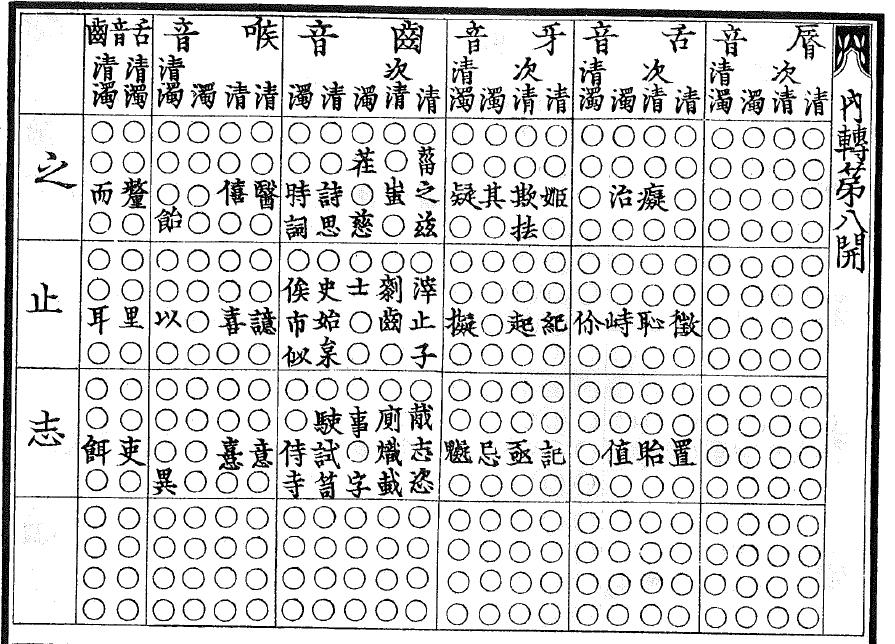
\includegraphics[width=.9\textwidth]{yunjing-i.jpg}
\end{figure}

「先侯」反,「先」字屬第四(\ref{fig:en})歸成「涑」字,又在第一(\ref{fig:uw}),蓋逐韻齒音中間二位屬照穿牀審禪字母,上下二位屬精清從心邪字母,侯字韻列第一行,故隨本韻定音也,餘準之。

\begin{figure}[H]
\centering
\label{fig:en}
\caption{\zhc{先}{-en}}
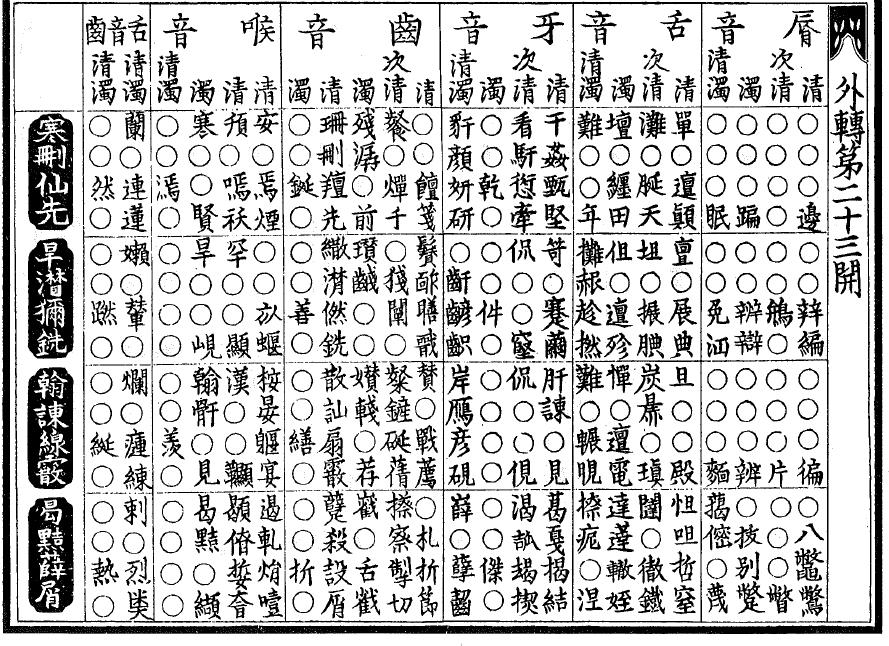
\includegraphics[width=.9\textwidth]{yunjing-an.jpg}
\end{figure}

\begin{figure}[H]
\centering
\label{fig:uw}
\caption{\zhc{侯}{-uw}}
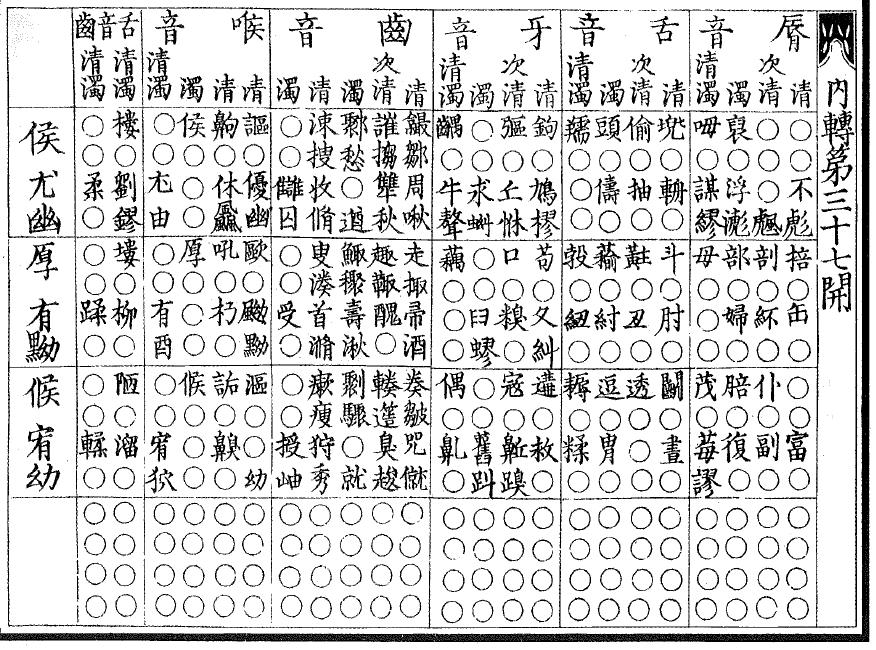
\includegraphics[width=.9\textwidth]{yunjing-uw.jpg}
\end{figure}

「諸氏」反、「莫蟹」反、「奴罪」反、「弭盡」反之類,聲雖去音,字歸上韻,並當從禮部韻就上聲歸字。

凡歸難字,橫音即所屬音四聲內任意取一字,橫轉便得之矣。今如「千竹」反「鼀」也(\ref{fig:uwng}),若取「嵩」字橫呼,則知平聲次清是為「樅」字,又以「樅」字呼下入聲則知「鼀」為「促」音(\ref{fig:owng})。但以二「冬」韻同音處觀之可見也。

\begin{figure}[H]
\centering
\label{fig:owng}
\caption{\zhc{冬}{-owŋ}}
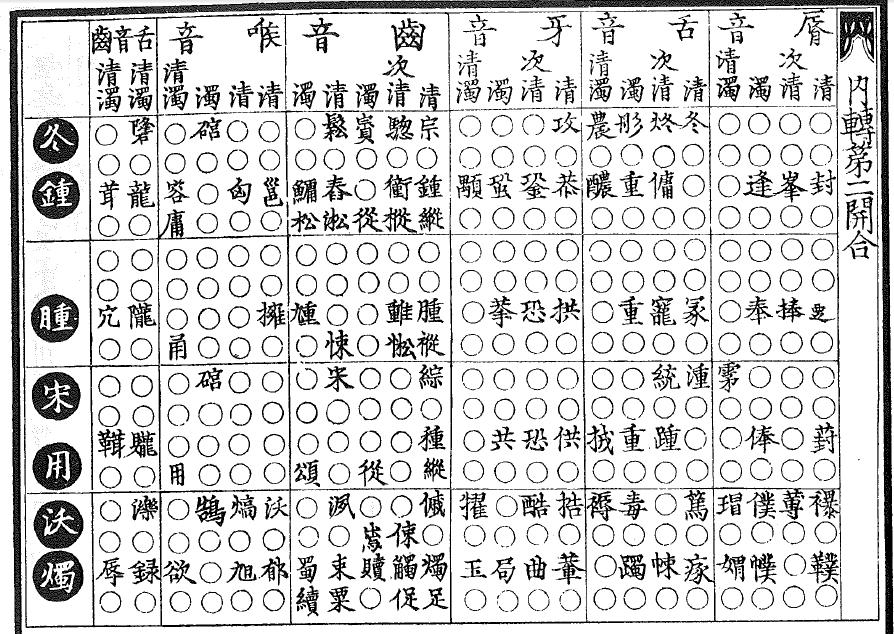
\includegraphics[width=\textwidth]{yunjing-owng.jpg}
\end{figure}
}
 \exercice{Indicate the MC transcription for all characters in pages of the Yunjing in Figures \ref{fig:uw} and \ref{fig:en}.}

 

\subsection{\zhc{平仄}{píngzè}} \label{sec:pingze}

Colour code: red: \zhc{\rouge{平}}{píng}, blue: \zhc{\bleu{仄}}{zè}, bold: \verte{both possible}.

\zhc{七言律詩}{qīyán lǜshī}, \zhc{杜甫}{Dù Fǔ}
\begin{itemize}
\item \zh{丞相祠堂何處尋,錦官城外柏森森。}

\ipa{\verte{dʑiŋ} \bleu{sjaŋH} \rouge{zi} \rouge{daŋ} \verte{ɣa} \bleu{tɕʰoH} \rouge{zim}}

\ipa{\verte{kimX} \rouge{kwan} \verte{dʑeŋ} \bleu{ŋwajH} \bleu{pæk} \rouge{ʂim} \rouge{ʂim}}

\item \zh{映階碧草自春色,隔葉黃鸝空好音。}

\ipa{\verte{ʔjæŋH} \rouge{kɛj} \bleu{pjæk} \bleu{tsʰawX} \bleu{dzijH} \rouge{tɕʰwin} \bleu{ʂik}}

\ipa{\verte{kɛk} \bleu{jep} \rouge{ɣwaŋ} \rouge{lje} \rouge{kʰuwŋ} \bleu{xawX} \rouge{ʔim}}

\item \zh{三顧頻煩天下計,兩朝開濟老臣心。}

\ipa{\verte{sam} \bleu{kuH} \rouge{bjin} \rouge{bjon} \rouge{tʰen} \bleu{ɣaX} \bleu{kejH}}

\ipa{\verte{ljaŋX} \rouge{ɖjew} \verte{kʰoj} \bleu{tsejX} \bleu{lawX} \rouge{dʑin} \rouge{sim}}

\item  \zh{出師未捷身先死,長使英雄淚滿襟。}

\ipa{\verte{tɕʰwit} \rouge{ʂij} \bleu{mjɨjH} \bleu{dzjep} \rouge{ɕin} \rouge{sen} \bleu{sijX}}

\ipa{\verte{ɖjaŋ} \bleu{ʂijX} \rouge{ʔjæŋ} \rouge{hjuwŋ} \bleu{lwijH} \bleu{manX} \rouge{kim}}
\end{itemize}
\section{Chinese Transcriptions of Sanskrit}

\subsection{\zhc{玄奘}{Xuánzàng}}
\subsubsection{Example from the \zhc{西域記}{Xīyùjì}}


\zh{\bleu{尼波羅}國周四千餘里,在雪山中。國大都城周二十餘里。山川連屬,宜穀稼,多花菓,出赤銅、犛牛、\rouge{命命鳥}。貨用赤銅錢。氣序寒烈,風俗險詖,人性剛獷,信義輕薄。無學藝,有工巧。形貌醜弊,邪正兼信。\bleu{伽藍}、天祠接堵連隅。僧徒二千余人,大小二乘,兼功綜習。外道異學,其數不詳。}

%一、光胄王制聲明論
\zh{王,\bleu{剎帝}\bleu{利栗呫婆}種也。志學清高,純信佛法。近代有王,號\bleu{鴦輸伐摩},(唐言\rouge{光胄}。)碩學聰睿,自制《\rouge{聲明論}》,重學敬德,遐邇著聞。}

\zh{都城東南有小水池,以人火投之,水即焰起。更投餘物,亦變為火。}

\zh{從此復還\bleu{吠舍釐}河,南渡\bleu{殑伽}河,至\bleu{摩揭陁}國。(舊曰\bleu{摩伽陁},又曰\bleu{摩竭提},皆訛也。中印度境。)}


\begin{itemize}

\item \zhc{尼波羅}{nepāla-}

\zhd{尼}{ɳij}\zhd{波}{pa}\zhd{羅}{la}

\item \zhc{命命}{jīvajīva-}
\item \zhc{伽藍}{saṃghārāma-} (abbreviation of \zh{僧伽藍摩})

\zhd{僧}{soŋ}\zhd{伽}{gja}\zhd{藍}{lam}\zhd{摩}{ma}
\item \zhc{剎帝利}{kṣatriya-}

\zhd{剎}{tʂʰæt}\zhd{帝}{tejH}\zhd{利}{lijH}
\item \zhc{栗呫婆}{licchava-}

\zhd{栗}{lit}\zhd{呫}{tɕʰep}\zhd{婆}{ba}
\item \zhc{鴦輸伐摩}{aṃśuvarman-}

\zhd{鴦}{ʔjaŋ}\zhd{輸}{ɕu}\zhd{伐}{bjot}\zhd{摩}{ma}
\item \zhc{聲明論}{śabdavidyāśāstra-}
\item \zhc{吠舍釐}{vaiśālī-}

\zhd{吠}{bjojH}\zhd{舍}{ɕæH}\zhd{釐}{li}
\item \zhc{殑伽}{gaṅgā-}

\zhd{殑}{giŋ}\zhd{伽}{gja}
\item \zhc{摩揭陁}{māgadha-}

\zhd{摩}{ma}\zhd{揭}{gjot}\zhd{陁}{da}; \zhd{摩}{ma}\zhd{伽}{gja}\zhd{陁}{da}; \zhd{摩}{ma}\zhd{竭}{gjot}\zhd{提}{dej}
\item \zhc{犛}{li ; mæw} `yak', Himalayan Wanderwort (OC *\ipa{rə}, *\ipa{mrə}, Tibetan \ipa{ɴbri} `female yak', Japhug \ipa{qambrɯ} `male yak', Skt \ipa{camara-, camarī-} `yak', cf \citealt{jacques16camara})
\end{itemize}
\subsubsection{Simple consonants}
Table \ref{tab:xz.initials}, from \citet{shixd83xuanzang}
%右上角有“*”号的字,见于圆明字轮和密咒的对音
\begin{table}[h]
\caption{Sanskrit consonants and MC initials (data from \citealt{shixd83xuanzang})} \label{tab:xz.initials}
\resizebox{\columnwidth}{!}{
\begin{tabular}{lllllll}
\midrule
\ipa{k} &	\zh{见} &	\zh{迦*宫恭枳*翅拘俱矩*句瞿稽雞蓟繫*计紧*} &	\zh{𩒣诘朅佉(溪纽)} \\
&&\zh{军捃建憍薑矜袈鸠金剑鞠吉*屈*讫羯*却劫} &\zh{健竭(群纽)}\\
\ipa{kh} &	\zh{溪} &	\zh{佉*企弃朅契} &	\zh{货汉(晓纽)} \\
\ipa{g} &	\zh{群} &	\zh{伽*祇窶瞿耆具惧*郡健乾揵乔殑毱局姞掘} &	\zh{拘(见纽)恒(匣纽)} \\
&&\zh{崛揭*笈} \\
\ipa{gh} &	\zh{群} &	\zh{键*祇窶瞿具勤犍伽*揭*} &	\zh{祛(溪纽)} \\
\ipa{n̄ (ng)} &	\zh{疑} &	\zh{御} &	\zh{} \\
\midrule
\ipa{c} &	\zh{照三} &	\zh{者*支脂旨至芝止*志珠主*注铸制真准準旃} &	\zh{} \\
&&\zh{栴战招遮*瞻占质折*酌*斫*} \\
\ipa{ch} &	\zh{穿三} &	\zh{绰*掣阐车*苫呫䶩} &	\zh{村(清纽)} \\
\ipa{j} &	\zh{禅三} &	\zh{闍*氏视豉时恃市*殊树逝誓慎鄯膳缮禅社赡} &	\zh{} \\
&&\zh{折*勺什*} \\
\ipa{ñ(jñ)} &	\zh{日} &	\zh{若攘尔} &	\zh{} \\
\midrule
\ipa{ṭ} &	\zh{知} &	\zh{吒*知胝置*竹哳*磔搩} &	\zh{侘搋(彻纽)荼雉(澄纽)} \\
&&&\zh{澍(照三)} \\
\ipa{ṭh} &	\zh{彻} &	\zh{搋*絺耻*祉𢯯侘诧* } &	\zh{吒(知纽)} \\
\ipa{ḍ} &	\zh{澄} &	\zh{荼*穉稚持陈阵茶择宅哒} &	\zh{铎度(定纽)} \\
\ipa{ḍh} &	\zh{澄} &	\zh{择*荼茶宅} &	\zh{搋(彻纽)} \\
\ipa{ṇ} &	\zh{娘,泥} &	\zh{拏*尼腻拿挐忸*痆匿*(娘纽) 儞笯怒弩泥揉} &	\zh{若攘(日纽)} \\
&&\zh{那诺(泥纽)} \\
\midrule
\ipa{t} &	\zh{端} &	\zh{䫂*都覩*堵妬蠹底*鞮低*帝*谛*旦颠刀多*埵*} &	\zh{知镇吒咤(知 纽)} \\
&&&\zh{茶(澄纽)} \\
&&\zh{蹬耽*点*咄呾*怛*德答*} \\
\ipa{th} &	\zh{透} &	\zh{他*土兔菟傥闼*铁託} &	\zh{陁陀(定纽)} \\
\ipa{d} &	\zh{定} &	\zh{柁*地*图弹度提*第檀坛陀*驮*陁惰堕墯头豆} &	\zh{茶仗阵陈(澄纽)} \\
&&\zh{昙达* 迭姪*絰*铎特踏叠} \\
\ipa{dh} &	\zh{定} &	\zh{达*地*杜*度提弹田陀驮*絰*沓柁} &	\zh{} \\
\ipa{n} &	\zh{泥,娘} &	\zh{娜*你*儞奴*笯埿泥耐㮈奈柰难那*橠南耨捺*} &	\zh{如任若(日纽)} \\
&&\zh{扌柰 诺纳*(泥纽)尼*腻昵*拏赁(娘纽)} \\
\midrule
\ipa{p} &	\zh{帮} &	\zh{跛*补谱*布闭*薜奔般半报波*播*簸卜毕荜㮿茇} &	\zh{毘掊跋薄(並 纽)芬(敷纽)} \\
&&\zh{钵*博弗卑鞞臂比蔽宾褒} \\
\ipa{ph} &	\zh{滂} &	\zh{颇*庀坡比蔽} & \\
\ipa{b} &	\zh{並} &	\zh{婆*菩*部*蒲*餔步*槃般畔渤*勃跋*频毗*} &	\zh{佛*梵(奉纽)} \\
\ipa{bh} &	\zh{並} &	\zh{薄*媲菩部*步陛槃畔叛婆*仆苾勃跋*毗鼻*鞞} &	\zh{浮(奉纽)} \\
\ipa{m} &	\zh{明} &	\zh{磨*弥弭*姥慕*迷谜*梅门闷*曼漫缦摩*魔茫*瞢*} &	\zh{物文(微纽)} \\
&&\zh{牟某母*茂贸穆木目藐蜜没秣末*沫*篾蔑莫*民} \\
\midrule
\ipa{y} &	\zh{喻四} &	\zh{也*夷已踰瑜渝逾*庾裕曳*延衍耶*夜*阎*盐琰剡} & \\
&&\zh{燄焰逸*洩药抴} \\
\ipa{l,r} &	\zh{来} &	\zh{洛*砢*离璃缡梨履*利*唎*釐理里缕*卢*嚧*鲁*} & \\
&&\zh{嚕虏路*露𡀔*黎戾丽*荔隸俪赖邻蔺兰烂连练劳} \\
&&\zh{罗*囉*逻*螺浪狼𩜁陵凌楞娄楼瑠岚览囕缆蓝滥} \\
&&\zh{禄栗律𢫫辣*剌*喇*络落勒拉*腊} \\
\ipa{v} &	\zh{奉, 並} &	\zh{缚*吠軬饭嚩*房防梵*凡*佛伐*罚*筏*栰(奉纽)} &\zh{波博弗(帮纽)} \\
&&\zh{避阰毗*鼻*频鞞槃婆*瓶跋薄(並纽)} \\
\midrule
\ipa{ś} &	\zh{审三} &	\zh{捨*施翅尸始*试输*戍世势扇*奢赊舍商赏饷蠰首} &	\zh{删沙(审二纽) } \\
&&\zh{兽室*设铄释式湿*葉摄} & \zh{珊(心纽)} \\
\ipa{ṣ} &	\zh{审二} &	\zh{沙*师使史愉崽鎩裟洒霜衫*瑟*杀*穑色歰*澀} & \\
\ipa{s} &	\zh{心} &	\zh{娑*斯徙玺私死*絮须苏*素*西犀信孙珊*骚些莎* } & \\
&&\zh{僧*薮三*叁参悉*窣*萨*塞*霫飒䬃} \\
\ipa{h} &	\zh{晓,匣} &	\zh{呬*希呼*虎醯汉诃*呵*兴亘喝*吸*噏(晓纽)} &	\zh{伽(群纽)} \\
&&\zh{嗑*纥*曷*睺护怙(匣纽)}\\
\midrule
\ipa{kṣ} &	\zh{穿二} &	\zh{羼*厕*刍*蒭叉*差创忏刹策} &	\zh{崎泣(溪纽)} \\
\ipa{ts} &	\zh{清} &	\zh{蹉*雌蹭} & \\
$\varnothing$ &	\zh{影} &	\zh{蓊*伊医乌隖邬坞瑿黳毉*翳哀蔼因印安案阿*𧙃* } & \\
&&\zh{鸯泱㹧*优沤菴庵罯*闇*郁壹鬰鬱嗢殟閼頞*遏恶垩} \\
\bottomrule
\end{tabular}}
\end{table}

\subsubsection{Clusters}

\begin{itemize}
\item \ipa{śr-}
\begin{itemize}
\item \zhc{沙门}{śramaṇa-} (old transcription)
\item \zhc{室罗摩拏洛迦}{śramaṇerikā-}

\zhd{室}{ɕit}\zhd{罗}{la}\zhd{摩}{ma}\zhd{拏}{næ}\zhd{洛}{lak}\zhd{迦}{kæ}
\end{itemize}
\item \ipa{sph-} \zhc{飒颇胝迦}{sphaṭika-}

\zhd{飒}{sop}\zhd{颇}{pʰa}\zhd{胝}{ʈij}\zhd{迦}{kæ}
\item \ipa{st-} \zhc{窣堵波}{stūpa-}

\zhd{窣}{swot}\zhd{堵}{tuX}\zhd{波}{pa} 
\item \ipa{st-} \zhc{塞建陀}{skandha-}

\zhd{塞}{sok}\zhd{建}{kjonH}\zhd{陀}{da} 
\end{itemize}
\subsection{\zh{不空} Amoghavajra} \label{sec:amoghavajra}

\citet{maspero1920changan}
\subsection{\zh{支婁迦讖} Lokakṣema }

\citet{karashima10lokakshema}
 
\bibliographystyle{unified}
\bibliography{bibliogj}

 \end{document}
 